% \iffalse meta-comment
%
% Copyright (C) 2021 by Geraldo Xexéo
%
% This file may be distributed and/or modified under the
% conditions of the LaTeX Project Public License, either
% version 1.3 of this license or (at your option) any later
% version. The latest version of this license is in:
%
% http://www.latex-project.org/lppl.txt
%
% and version 1.3 or later is part of all distributions of
% LaTeX version 2005/12/01 or later.
%
% \fi
%
%
%\iffalse
%<package>\NeedsTeXFormat{LaTeX2e}
%<package>\def\tr@version{v0.4}
%<package>\ProvidesPackage{task-report}[2021/05/31 \tr@version task-report]
%<*driver>
\documentclass{ltxdoc}
\usepackage[T1]{fontenc}
\usepackage[utf8]{inputenc}
\usepackage{lmodern}
\usepackage{csquotes}
\usepackage[brazilian,english]{babel}
\usepackage{datetime}
\usepackage{graphicx}
\usepackage{indentfirst}
\setlength{\parskip}{0.5em}
\usepackage{marvosym}
\usepackage[backend=biber,style=alphabetic,natbib]{biblatex}
\usepackage[editing]{coop-writing}
\usepackage{task-report}
\setlength{\cfttasksnumwidth}{25pt}
\usepackage{hyperref}
\cwnamedef{xexeo}{red}{Xexéo}
%
\EnableCrossrefs
\CodelineIndex
\RecordChanges
%
\DoNotIndex{\def,\long,\edef,\xdef,\gdef,\let,\global}
\DoNotIndex{\begin,\AtEndDocument,\newcommand,\newcounter,\stepcounter}
\DoNotIndex{\immediate,\openout,\closeout,\message,\typeout}
\DoNotIndex{\section,\scshape,\arabic}
%
%
%
\title{Task Report \taskreportversion}
\author{Geraldo Xexéo}
\date{\today\ - \ \currenttime}
\GetFileInfo{task-report.sty}
%
\makeindex
\MakeShortVerb{\|}
\begin{document}
    \DocInput{task-report.dtx}
    \newpage
    \PrintChanges
    \newpage
    \PrintIndex
    \newpage
    \listoftasks
\end{document}
%</driver>
% \fi
%
% \CheckSum{151}
%
% \CharacterTable
%  {Upper-case    \A\B\C\D\E\F\G\H\I\J\K\L\M\N\O\P\Q\R\S\T\U\V\W\X\Y\Z
%   Lower-case    \a\b\c\d\e\f\g\h\i\j\k\l\m\n\o\p\q\r\s\t\u\v\w\x\y\z
%   Digits        \0\1\2\3\4\5\6\7\8\9
%   Exclamation   \!     Double quote  \"     Hash (number) \#
%   Dollar        \$     Percent       \%     Ampersand     \&
%   Acute accent  \'     Left paren    \(     Right paren   \)
%   Asterisk      \*     Plus          \+     Comma         \,
%   Minus         \-     Point         \.     Solidus       \/
%   Colon         \:     Semicolon     \;     Less than     \<
%   Equals        \=     Greater than  \>     Question mark \?
%   Commercial at \@     Left bracket  \[     Backslash     \\
%   Right bracket \]     Circumflex    \^     Underscore    \_
%   Grave accent  \`     Left brace    \{     Vertical bar  \|
%   Right brace   \}     Tilde         \~}
%
% \changes{v0.1}{2021/05/31}{First version}
% \changes{v0.2}{2021/05/31}{User can create own states}
% \changes{v0.3}{2021/05/31}{List of Tasks}
% \changes{v0.4}{2021/06/01}{Allows redefining field names}
%\maketitle
%
% \tableofcontents
%
%\section{Introduction}
%
% This package supports the maintenance and report of a task list..
%
%
% \section{How to use task-report}
%
% |task-report| is available as open source at \url{https://github.com/xexeo/task-report}. The stable distribution is in the folder |dist|, while the lastest, and unstable, will be in the root folder.
%
% The only file you really need, besides this manual, is
% |task-report.sty|. This should be in your \LaTeX\   path, such as in the same folder that your main |.tex| file.
%
% You can make suggestions, complain about bugs, and request features using GitHub's ``Issues'' feature, in \url{https://github.com/xexeo/task-report/issues} (you must be signed in).
%
% \subsection{Using from Overleaf}
%
% The best way to use |task-report| inside Overleaf is to link
% the distributed style file through its URL. To do that, inside your project, select first ``Upload''. An ``Add files'' window will appear, then select ``From Externa URL'' and enter \url{https://raw.githubusercontent.com/xexeo/task-report/main/dist/task-report.sty} as ``URL to fetch the file from'' and ``task-report'' as ``File Name in This Project'', as in Figure \ref{fig:overleaffileurl}.
%
%\begin{figure}[tbh]
%    \centering
%    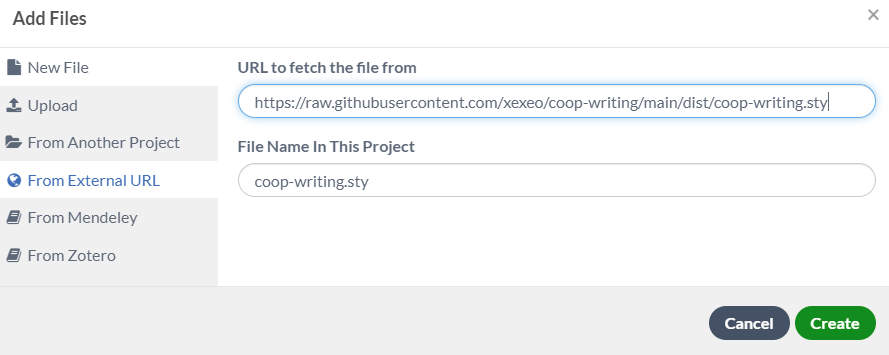
\includegraphics[width=0.9\linewidth]{images/overleaffileurl}
%    \caption{How to link a task-report.sty file in your project folder in Overleaf to the official distribution.}
%    \label{fig:overleaffileurl}
%\end{figure}
%
%
% \section{Package Options}
%
% There are no package options up to now
%
% \subsection{General behavior}
%
%
%\section{Version}
%
% It is possible that the user wants to know the version
% being used. We provide two commands for it.
%
% \DescribeMacro{\taskreportversion}
% Provides the current version
%
% \DescribeMacro{\printtaskreportversion}
% Provides name and version
%
%
% |\taskreportversion| was used in the title of this article. The current version is \taskreportversion.
%
% If needed, the second macro prints also the name of the
% package:
%
%|\printtaskreportversion|
%
% will result in:
%
%\printtaskreportversion
%
% Please state the version when reporting bugs.
%
%
% \section{Usage}
%
% \DescribeMacro{\trtask}
% This is the main macro for the package.
%|\trtask|\oarg{status}\marg{name}\marg{when-assigned}
% \marg{who-assigned}\marg{to-who-assigned}
% \marg{why}
% \marg{when-done}
% \marg{extra-text}
%
% Altough it has 7 mandatory parameters, all of them can be empty.
%
% There are 5 possible states that are associated with a color (\textit{default color}): todo (red), doing(yellow), tocheck (cyan), checking (blue), and done(green). There is a pseudo-state other (black) that will be the color of any other word used of a state. Colors belong to the |xcolor| package and are configurable, as explained in section \ref{sec:conf}.
%
% The example:
%\begin{verbatim}
%\trtask[todo]{Mage coffe}{\today}{Geraldo Xexéo}{}{}{}{Please do the coffe strong}
%\trtask[doing]{Drink a coffe}{June, 1st 2021}{The Boss}{The Worker}{}{}{}
%\trtask[tocheck]{Roast the beef}{June, 1st 2021}{The Boss}{The Worker}{\today}{}{Rare, please}
%\trtask[checking]{Drink another beer}{June, 1st 2021}{The Boss}{The Worker}{\today}{}{Please check if you have age to drink in your country. If not, drink orangejuice.}
%\trtask[done]{Drink a beer}{\today}{The Boss}{The Worker}{\today}{}{}
%\trtask{}{}{}{}{}{}{}
%\trtask[done]{}{}{}{}{}{}{}
%\trtask{Grab a hot-dog}{3}{4}{5}{6}{7}{A hot dog must be done with bread and sausage}
%\end{verbatim}
% generates:
%
%\trtask[todo]{Make coffe}{\today}{Geraldo Xexéo}{}{}{}{Please do the coffe strong}
%\trtask[doing]{Drink a coffe}{June, 1st 2021}{The Boss}{The Worker}{}{}{}
%\trtask[tocheck]{Roast the beef}{June, 1st 2021}{The Boss}{The Worker}{}{\today}{Rare, plese}
%\trtask[checking]{Drink another beer}{June, 1st 2021}{The Boss}{The Worker}{}{\today}{Please check if you have age to drink in your country. If not, drink orangejuice.}
%\trtask[done]{Drink a beer}{\today}{The Boss}{The Worker}{Because I want}{\today}{}
%\trtask{}{}{}{}{}{}{}
%\trtask[done]{}{}{}{}{}{}{}
%\trtask[arg 1]{arg 2}{arg 3}{arg 4}{arg 5}{arg 6}{arg 7}{arg 8}
%
%
% \subsection{Configuration Options}
%\label{sec:conf}
%
% \subsubsection{Configuring Colors}
%
% \DescribeMacro{\trsetboxcolors}
%% Set the colors for the 6 types of standard states
% Black otherwise.
%
% |\trsetboxcolors|\marg{todo-color}\marg{doing-color}\marg{tocheck-color}\marg{checking-color}\marg{done-color}\marg{other-color}
%
% The example:
%
%\begin{verbatim}
%\trsetboxcolors{magenta}{purple}{orange}{pink}{lime}{pink}
%
%\trtask[todo]{Drink a coffe}{\today}{The Boss}{The Worker}%
%{To keep awake}{\today}{Coffe must be strong and add 1 spoon of sugar}
%\trtask[doing]{Drink a coffe}{\today}{The Boss}{The Worker}%
%{To keep awake}{\today}{Coffe must be strong and add 1 spoon of sugar}
%\trtask[tocheck]{Drink a coffe}{\today}{The Boss}{The Worker}%
%{To keep awake}{\today}{Coffe must be strong and add 1 spoon of sugar}
%\trtask[checking]{Drink a coffe}{\today}{The Boss}{The Worker}%
%{To keep awake}{\today}{Coffe must be strong and add 1 spoon of sugar}
%\trtask[done]{Drink a coffe}{\today}{The Boss}{The Worker}%
%{To keep awake}{\today}{Coffe must be strong and add 1 spoon of sugar}
%\trtask{Drink a coffe}{\today}{The Boss}{The Worker}%
%{To keep awake}{\today}{Coffe must be strong and add 1 spoon of sugar}
%\end{verbatim}
%
% generates:
%
%\trsetboxcolors{magenta}{purple}{orange}{pink}{lime}{pink}
%
%\trtask[todo]{Drink a coffe}{\today}{The Boss}{The Worker}%
%{To keep awake}{\today}{Coffe must be strong and add 1 spoon of sugar}
%\trtask[doing]{Drink a coffe}{\today}{The Boss}{The Worker}%
%{To keep awake}{\today}{Coffe must be strong and add 1 spoon of sugar}
%\trtask[tocheck]{Drink a coffe}{\today}{The Boss}{The Worker}%
%{To keep awake}{\today}{Coffe must be strong and add 1 spoon of sugar}
%\trtask[checking]{Drink a coffe}{\today}{The Boss}{The Worker}%
%{To keep awake}{\today}{Coffe must be strong and add 1 spoon of sugar}
%\trtask[done]{Drink a coffe}{\today}{The Boss}{The Worker}%
%{To keep awake}{\today}{Coffe must be strong and add 1 spoon of sugar}
%\trtask{Drink a coffe}{\today}{The Boss}{The Worker}%
%{To keep awake}{\today}{Coffe must be strong and add 1 spoon of sugar}
%
%
%\trsetboxcolors{red}{yellow}{cyan}{blue}{green}{black}
%
%
% \subsection{Changing Field Names}
%
% You can change all field names with command \DescribeMacro{\trsetfieldsnames}.
%
%
% |\trsetfieldsnames|\marg{status}\marg{assigned}
% \marg{from}\marg{to}
% \marg{done}\marg{why}
%
%
% For example:
%
%\begin{verbatim}
%\trsetfieldsnames{Stage}{Demand date}{Who asked for}{To who}{Ready in}{Reasons}
%\trtask[done]{Drink a coffe}{\today}{The Boss}{The Worker}%
%{To keep awake}{\today}{Coffe must be strong and add 1 spoon of sugar}
%\end{verbatim}
%
% generates:
%
%\trsetfieldsnames{Stage}{Demand date}{Who asked for}{To who}{Ready in}{Reasons}
%\trtask[done]{Drink a coffe}{\today}{The Boss}{The Worker}%
%{To keep awake}{\today}{Coffe must be strong and add 1 spoon of sugar}
%
% This command can be used to internationalization.
%
%\trsetfieldsnames{Status}{Assigned in}{From}{To}{Done in}{Rationale}
%
% \subsection{Creating New States}
%
% Users can create their own state using  \DescribeMacro{\traddstatecolor}
%
% |\traddstatecolor|\marg{state}\marg{color}
%
% For example:
%
%\begin{verbatim}
%\traddstatecolor{waiting}{teal}
%\trtask[waiting]{Drink a coffe}{\today}{The Boss}{The Worker}%
%{To keep awake}{\today}{Coffe must be strong and add 1 spoon of sugar}
%\end{verbatim}
%
% generates:
%
%\traddstatecolor{waiting}{teal}
%\trtask[waiting]{Drink a coffe}{\today}{The Boss}{The Worker}%
%{To keep awake}{\today}{Coffe must be strong and add 1 spoon of sugar}
%
% \section{The List of Tasks}
%
% \DescribeMacro{\listoftasks}
% A list of tasks can be generated with the command:
%
% |\listoftasks|
%
%
% Its title can be changed with the command:
%
% |\trsettasklisttitle|\marg{new-title}
%
% The command:
%
% |\setlength{\cfttasksnumwidth}{25pt}|
%
% from package |tocloft| can be used to set the space used by
% the section indicator.
%
%
%
%\section{Warnings}
% This package uses another package that changes \LaTeX's standard behavior for summary and lists. When you use it, you must explicitly change pages with |\newpage|
% before |\tableofcontents| or similar commands.
%
% \section{Implementation}
%
% \StopEventually{End of Code}
%
% \subsection{Required Packages}
%
%
%\begin{itemize}
%    \item |mdframed| makes the frame aroung tasks
%    \item |etoolbox| command ifstringempty
%    \item |tocloft|  create the list of tasks
%\end{itemize}
%
%    \begin{macrocode}
\RequirePackage{tcolorbox}%
\RequirePackage{etoolbox}%
\RequirePackage{tocloft}
%    \end{macrocode}
%
% \subsection{Access to the current version}
% We provide some macros for the user to know the version being used.
% \begin{macro}{\taskreportversion}
% Provides current version of coop-writing
%    \begin{macrocode}
\newcommand{\taskreportversion}{\tr@version}%
%    \end{macrocode}
% \end{macro}
%
% \begin{macro}{\printtaskreportversion}
% Provides package name and version
%    \begin{macrocode}
\newcommand{\printtaskreportversion}{task-report v. \taskreportversion}%
%    \end{macrocode}
% \end{macro}
%
% \subsection{Color Management for States}
%
% \subsection{Defining States Through a Simulated List}
%
% \begin{macro}{\traddstatecolor}
% \begin{macro}{\usestatecolor}
%
% Inserts states and their colors in a simulated list and uses them
%
%    \begin{macrocode}
\newcommand{\traddstatecolor}[2]{%
    \@ifundefined{\string\color@#2}%
    {%
        \message{#2 not defined}%
        \expandafter\ERROR%
    }%
    {%
        \expandafter\gdef\csname tr@astate@\detokenize{#1}\endcsname{#2}%
}%
}%
%
\def\tr@usestatecolor#1{%
    \ifcsname tr@astate@\detokenize{#1}\endcsname%
    \csname tr@astate@\detokenize{#1}\expandafter\endcsname%
    \else%
\tr@astate@other%
    \fi%
}%
%    \end{macrocode}
% \end{macro}
% \end{macro}
%
% \begin{macro}{\trsetboxcolors}
%
% Set the colors for the 6 types of standard states
% Black otherwise.
%
% |\trsetboxcolors|\marg{todo-color}\marg{doing-color}
% \marg{tocheck-color}\marg{checking-color}
% \marg{done-color}\marg{other-color}
%
%    \begin{macrocode}
\newcommand{\trsetboxcolors}[6]{%
\traddstatecolor{todo}{#1}
\traddstatecolor{doing}{#2}
\traddstatecolor{tocheck}{#3}
\traddstatecolor{checking}{#4}
\traddstatecolor{done}{#5}
\traddstatecolor{other}{#6}
}%
%    \end{macrocode}
% \end{macro}
% \subsection{Standard Colors}
%
% Sets the standard colors for the standard states
%
%    \begin{macrocode}
\trsetboxcolors{red}{yellow}{cyan}{blue}{green}{black}
%    \end{macrocode}
%
%
% \subsection{Managing The Fields Names}
%
% \begin{macro}{\traddfieldname}
% \begin{macro}{\tr@usesfieldname}
%
% Define field names - does not create a new field
%
%    \begin{macrocode}
\newcommand{\traddfieldname}[2]{%
    \expandafter\gdef\csname tr@fieldnames@\detokenize{#1}\endcsname{#2}%
}%
%
\def\tr@usesfieldname#1{%
    \ifcsname tr@fieldnames@\detokenize{#1}\endcsname%
    \csname tr@fieldnames@\detokenize{#1}\expandafter\endcsname%
    \else%
Missing Field Name%
    \fi%
}%
%    \end{macrocode}
% \end{macro}
% \end{macro}
%
% \begin{macro}{\trsetboxcolors}
%
% Set the colors for the 6 types of standard states
% Black otherwise.
%
% |\trsetfieldsnames|\marg{status}\marg{assigned}
% \marg{from}\marg{to}
% \marg{done}\marg{why}
%
%    \begin{macrocode}
\newcommand{\trsetfieldsnames}[6]{%
    \traddfieldname{status}{#1}
    \traddfieldname{assigned}{#2}
    \traddfieldname{from}{#3}
    \traddfieldname{to}{#4}
    \traddfieldname{done}{#5}
    \traddfieldname{why}{#6}
}%
%    \end{macrocode}
% \end{macro}
% \subsection{Standard Field Names}
%
% Sets the standard text for the fields
%
%    \begin{macrocode}
\trsetfieldsnames{Status}{Assigned in}{From}{To}{Done in}{Rationale}
%    \end{macrocode}
%
%
% \begin{macro}{\tr@currentboxcolor}
%
% The dirt trick of using a global variable to
% store a value
%
%    \begin{macrocode}
\def\tr@currentboxcolor{\tr@usestatecolor{other}}%
%    \end{macrocode}
% \end{macro}
%
%
%
% \begin{macro}{\trstatuscolor}
%
% Select the color based on the state
%
% |\trstatuscolor|\marg{state}
%
%    \begin{macrocode}
\newcommand{\trstatuscolor}[1]%
{%
\ifblank{#1}%
{%
\def\tr@currentboxcolor{\tr@usestatecolor{other}}%
}%
{%
\def\tr@currentboxcolor{\tr@usestatecolor{#1}}%
}%
}%
%    \end{macrocode}
% \end{macro}
%
%
% \section{List of Tasks}
%    \begin{macrocode}
\newcommand{\trsettasklisttitle}[1]{%
    \def\trlisttasks{#1}%
}%
\trsettasklisttitle{List of Tasks}%
%% cria a lista, depende do pacoto tcloft
\@ifundefined{chapter}%
{\newlistof[section]{tasks}{trt}{\trlisttasks}}%
{\newlistof[chapter]{tasks}{trt}{\trlisttasks}}%
%    \end{macrocode}
%
% \subsection{Declaring Tasks}
%
% \subsubsection{Helpers}
%
% \begin{macro}{\trstatus}
% \begin{macro}{\trwhen}
% \begin{macro}{\trwhy}
% \begin{macro}{\trwho}
%
% Helpers to build the task
%
%    \begin{macrocode}
\newcommand{\trstatus}[2][\tr@usesfieldname{status}]{%
    \textbf{#1}: #2%
}%
\newcommand{\trwhen}[2][\tr@usesfieldname{assigned}]{%
    \textbf{#1}: #2%
}%
\newcommand{\trwho}[2][\tr@usesfieldname{to}]{%
    \textbf{#1}: #2%
}%
\newcommand{\trwhy}[2][\tr@usesfieldname{why}]{%
    \textbf{#1}: #2%
}%
%
%    \end{macrocode}
% \end{macro}
% \end{macro}
% \end{macro}
% \end{macro}
%
% \subsubsection{Main task macro}
%
% \begin{macro}{\trtask}
%
%  Describes a task
%
%|\trtask|\oarg{status}\marg{name}\marg{when-assigned}
%\marg{who-assigned}\marg{to-who-assigned}\marg{why}\marg{when-done}\marg{extra-text}
%
% For example:
%\begin{verbatim}
%\trtask[Help students organize]{doing}
% {Prepare a \LaTeX\ style to support task report}
% {2021-05-31}{Xexéo}{Geraldo Xexéo}{}
%\end{verbatim}
%
% generates:
%
%\trtask[doing]{Prepare a \LaTeX\ style to support task report}
% {2021-05-31}{Xexéo}{Geraldo Xexéo}{Help students organize}
% {not yet}{This is an idea to help understanding the work being done}
%
%    \begin{macrocode}
%  [status] , what, when-assigned, from-who, to-who, why, when-done, extra
\newcommand{\trtask}[8][]{%
    \par%
    \ifblank{#2}{
    \def\trtask@temp{Task without a name}%
    }%
    {%
    \def\trtask@temp{#2}%
    }%
    \refstepcounter{tasks}%
    \addcontentsline{trt}{tasks}{\protect\numberline{\thetasks}{\trtask@temp}}%
    \trstatuscolor{#1}%
    \begin{tcolorbox}[title=\textbf{\trtask@temp},%
         colback=\tr@currentboxcolor!5!white,%
         colframe=\tr@currentboxcolor!75!black%
        ]%
        \ifblank{#1}{}%
        {%
            \trstatus{#1}\newline%
        }%
        \ifblank{#3}{}%
        {%
            \trwhen{#3}\newline%
        }%
        \ifblank{#4}{}%
        {%
            \trwho[\tr@usesfieldname{from}]{#4}\newline%
        }%
        \ifblank{#5}{}%
        {%
            \trwho{#5}\newline%
        }%
        \ifblank{#6}{}%
        {%
            \trwhy{#6}\newline%
        }%
        \ifblank{#7}{}%
        {%
            \trwhen[\tr@usesfieldname{done}]{#7}\newline%
        }%
        \ifblank{#8}{}%
        {\tcblower%
        #8%
        }%
    \end{tcolorbox}%
}%
%    \end{macrocode}
% \end{macro}
%
%
%
%
% \Finale
%
% \endinput
% Local Variables:
% mode: doctex
% TeX-master: t
% End:
